\input{vorlage_light}
\graphicspath{./bilder/}

%Für diese Version des Dokuments spezielle Anpassungen
\newcommand{\lat}[2]{(\textit{Lateinisch \glqq{}#1\grqq{} = #2})}
\newcommand{\merk}[1]{\glqq{}\textit{#1}\grqq{}}


\lohead{\includesvg[height=8mm]{bilder/ba_glauchau_logo}}

\begin{document}
\frontmatter

\title{Vorlesungsskript Ingenieursmathematik 4DE19-1-IMA}

\author{Dominic Sczyrba}
\date{14. September 2021}

\maketitle
\tableofcontents

\mainmatter
\setlength{\mathindent}{0cm}

\section{Allgemeine Grundlagen Elementarer Mathematik}
    \subsection{Axiome, Definitionen und Sätze (vgl. ET-LV)}
        \label{sec:grundlagen}
        \subsubsection{Axiome}
            \begin{itemize}[leftmargin=*]
                \item Grundannahmen die aus der unmittelbaren Anschauung resultieren
                \item Einleichtentes Prinzip, das keines Beweises bedarf
                \item Formale Eigenschaft
                \item Eine unabgeleitete Aussage
            \end{itemize}
            \underline{Beispiele:}
            \begin{itemize}[leftmargin=*]
                \item Newtonsche Axiome
                \item Grundgesetz der Elektrostatik
                \item Kommutativgesetz \lat{commutare}{vertauschen}\\
                    \vspace{-0.8cm}
                    \begin{eqnarray*}
                        a \ +     \ b &=& b \ +     \ a \\
                        a \ \cdot \ b &=& b \ \cdot \ a \\
                        a \ \land \ b &=& b \ \land \ a \\
                        a \ \lor  \ b &=& b \ \lor  \ a
                    \end{eqnarray*}
                \item Assoziativgesetz  \lat{soziare}{zusammengehörig}
                \item Distributivgesetz \lat{distribuere}{verteilen}
                \item Geometrie - Euklid \\
                    \merk{Durch einen Punkt außerhalb einer Gerade gibt es nur eine Gerade, die sich mit der Gegebenen nicht schneidet.}
                    \\ (Zeichnung parallele Linien und Zeichnung gekrümmte Ebene einfügen)
            \end{itemize}
        \subsubsection{Definitionen}
            \begin{itemize}[leftmargin=*]
                \item (sinnvolle) Festlegungen
                \item ebenfalls nicht beweisbar
            \end{itemize}
            \underline{Beispiele:}
            \begin{itemize}[leftmargin=*]
                \item $\varrho = \frac{dQ}{dV}$
                \item $i = \frac{d}{dt} Q(t)$
                \item $R = \frac{U}{I}$
                \item   \begin{tabular}[t]{l l}
                        Potenzieren     &  $a^b  \ \equiv \ \overbrace{a \cdot a \cdot a \cdot a \cdot \ldots}^{b \text{-Faktoren}} $ \\
                                        &  $2^{4}\ \equiv \ {2 \cdot 2 \cdot 2 \cdot 2 \cdot 2 \cdot = 32}$ \\ 
                                        &  $a^0 \ = \ 1$ \\
                        $\implies$ Idee: &  $a^b = \underbrace{a \cdot a \cdot a \cdot a}_{b \text{-Faktoren}} \cdot 1$ \\  
                        \end{tabular}
            \end{itemize}
        \subsubsection{Sätze}
            \begin{itemize}[leftmargin=*]
                \item wahrheitsfähige und beweispflichtige Aussagen
            \end{itemize}
            \underline{Beispiel: } Wenn eine Zahl durch $8$ teilbar ist, dann ist sie auch durch $4$ teilbar. 

            \begin{tabular}{@{}l l}
                Beweis: & Es sei $x\in\mathbb{N}$, wenn $\frac{x}{8} = y$ und $y\in\mathbb{N}$. \\
                & $\implies \frac{x}{2 \cdot 4} = y | \cdot 2$ dann ist $\frac{x}{4} = 2 \cdot y$ d.h. ebenfalls $\in\mathbb{N}$. \\
            \end{tabular}

            \underline{$\Rightarrow$ Merke:} \merk{Formeln gibt es weder in Mathematik noch in Physik.}
    \subsection{Mengenlehre}
        lt. Georg Cantor (1845 - 1918)
            \subsubsection{Begriffe und Darstellungen}
                \underline{Definition Menge:} \merk{Zusammenfassung von bestimmten wohlunterscheidbaren Objekten (Elementen) unserer Anschauung oder unseres Denkens}

                \underline{Beispiele:}
                    \begin{itemize}[leftmargin=*]
                        \item Menge aller Computer
                        \item Menge aller Programmiersprachen
                        \item Menge aller Lösungen einer Gleichung
                        \item Menge aller natürlichen Zahlen
                        \item Menge aller Gedanken
                    \end{itemize}

                \underline{Wichtig:}
                    \begin{itemize}[leftmargin=*]
                        \item mindestens \bfseries eine \mdseries gemeinsame Eigenschaft
                        \item für die Entscheidung, ob ein Element zu einer Menge gehört oder nicht, gibt es die Symbolik: \\
                            $x \in M \quad x \notin M $ \} ist stets eindeutig (deterministisch)
                        \item \underline{Achtung:} Die Elemente einer Menge müssen nicht geordnet sein, z.B. Die Menge aller Ebenenfiguren (Kreise, Quadrate, Rechtecke)
                        \item \underline{Darstellungsformen:}
                        \item[] \begin{tabular}{@{}l p{9cm}}
                            a) aufzählende Form             & $M_1 = \{1, \ 2, \ 3\} $  \\
                                                            & $M_2 = \{\blacklozenge, \ \blacksquare, \ \blacktriangle \} $  \\
                                                            & $M_3 = \{\text{Max}, \ \text{Moritz}\} $ \\
                                                            & $M_4 = \{true, \ false\} $ \\
                            b) fest eingeführte Buchstaben  &  $ x \ \in \ \mathbb{N}$\\ 
                            c) beschreibende Form           & $A = \{a \underbrace{|}_{mit} a \text{~besitzt die Eigenschaft~} E\}$\\
                                                            & $B = \{b | b \text{~ist ein weiblicher Vorname} \} $ \\
                                                            & $C = \{c | c \text{~ist eine gerade Zahl} \} $ \\
                                                            & $D = \{d \in \mathbb{N} | d^2 - 3d + 2 = 0 \} $\\
                            d) Venn - Diagramm              & Skizze vom Venn Diagramm einfügen \\
                            e) Zahlenstrahl                 & Skizze vom Zahlenstrahl \\
                            f) geometrische Gebilde         & Ein Kreis ist die Menge aller Punkte, die in der Ebene von einem Mittelpunkt $M$ den gleichen Abstand $r$ besitzen.\\
                            g) als Tabelle                  & DE19 \quad $\underbrace{\text{Matrikelnummer \ Name \ Vorname}}_{\text{eine Relation}}$ \\
                            \end{tabular}
                        \item \underline{Kennzeichnung der leeren Menge}
                        \item[] $M \ = \ \{\}$ oder $M \ = \ \varnothing$
                        \item \underline{Kennzeichnung von endlicher / unendlicher Menge}
                        \item[] $ M \ = \ \{ 1,\ 2,\ 3, \ 4, \ \ldots, \ 20\} $ \\
                                $ M \ = \ \{ 1,\ 2,\ 3, \ 4, \ \ldots \} $
                        \item \underline{Kennzeichnung der Einheitsmenge $\mathbb{E}$}
                        \item[] Venn-Diagramm mit Einheitsmenge einfügen
                        \item \underline{Kennzeichnung der Anzahl der Elemente}
                        \item[] $|m| $ \\ $|\{\rhd,\ \triangleleft,\ \triangleright \}| \ = \ 3$
                    \end{itemize}
                \subsubsection{Beziehungen zwischen Mengen}
                \begin{itemize}[leftmargin=*]
                    \item[a)] $A = B$ \quad (auch $A\equiv B$) z.B. $\{1, 2\} = \{2, 1\}$ 
                    \item[b)] $\underbrace{A\subseteq B}_{Teilmenge}$ bzw. $\underbrace{A \subset B}_{echte~Teilmenge}$
                    \item[] z.B. $\{1,\ 2\} \subset \{1,\ 5,\ 2\}$
                    \item[] 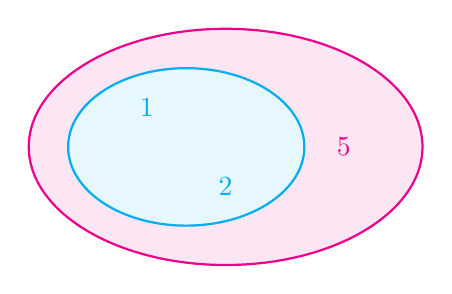
\begin{tikzpicture}
                        \filldraw[color=magenta, fill=magenta!10, thick] (0,0) ellipse (2.5 and 1.5);
                        \filldraw[color=cyan, fill=cyan!10, thick] (-0.5, 0) ellipse (1.5 and 1.0);
                        \coordinate[label=center:$\textcolor{cyan}{2}$] (M) at (0, -0.5);
                        \coordinate[label=center:$\textcolor{cyan}{1}$] (M) at (-1, 0.5);
                        \coordinate[label=center:$\textcolor{magenta}{5}$] (M) at (1.5, 0);
                        \end{tikzpicture} 
                    \item[] \underline{Satz:} Wenn $A \subseteq B$ und $B \subseteq A \Leftrightarrow A = B$
                    \item[c)] Komplementmenge (Bezugsmenge oder Grundmenge)
                    \item[] 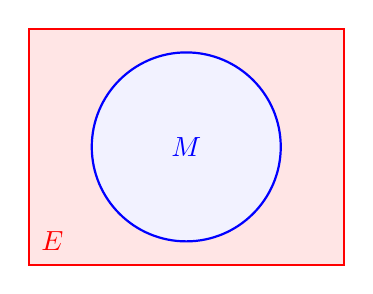
\begin{tikzpicture}
                        \filldraw[color=red,fill=red!10, thick] (0, 0) rectangle (4, 3);
                        \draw[color=blue, fill=blue!5, thick] (2, 1.5) circle (1.2);
                        \coordinate[label=center:$\textcolor{blue}{M}$] (M) at (2, 1.5);
                        \coordinate[label=center:$\textcolor{red}{E}$] (E) at (0.3, 0.3);
                        \end{tikzpicture}\quad \textcolor{red}{$\overline{\textcolor{blue}{M}}^E$} Komplement zu \textcolor{blue}{M}. bzgl. \textcolor{red}{E}
                    \item[d)] Potenzmenge  
                    \item[] Potenzmenge $P(M)$ $\Rightarrow$ Menge aller Teilmengen von $M$
                    \item[] \underline{Beispiel:}\hphantom{sss} $M = \{1, \ 2, \ 3\}$
                    \item[] \hphantom{Beispiel}\hphantom{sss} $M = \Big\{\{1\}, \{2\}, \{3\}, \{1, 2\}, \{1, 3\}, \{2, 3\}, \{1, 2, 3\}\Big\} + \varnothing $
                    \item[] \underline{Satz:} Wenn $n \ = \ |m|$, dann $|P(m)| \ = \ 2^n$
                \end{itemize}
            \subsubsection{Mengenoperationen}
                \begin{itemize}[leftmargin=*]
                    \item 
\end{document}